\documentclass[11pt]{article}
\usepackage{graphicx}
\usepackage{hyperref}
%\usepackage{appendix}
\usepackage{amsmath}
\usepackage{amsthm}
\usepackage{amssymb}
\usepackage{float}
\usepackage{commath}
\usepackage{booktabs}
\renewcommand{\arraystretch}{1.2}
\usepackage{siunitx}
\sisetup{detect-all}
\usepackage{listings}
\usepackage{color} %red, green, blue, yellow, cyan, magenta, black, white
\definecolor{mygreen}{RGB}{28,172,0} % color values Red, Green, Blue
\definecolor{mylilas}{RGB}{170,55,241}
\usepackage[a4paper,margin=20mm]{geometry}
\numberwithin{equation}{section}
\setlength{\parskip}{\baselineskip}
\setlength{\parindent}{0pt}
\hypersetup{
    colorlinks=true,
    linkcolor=black,
    filecolor=black,      
    urlcolor=black,
    citecolor=black
}
\urlstyle{same}
\begin{document}
\title{\textbf{UCL Mechanical Engineering 2020/2021}\\MECH0013 Final Assessment}
\author{NCWT3}
\maketitle
\tableofcontents
\listoffigures
\section{Question 1}
\subsection{i}
Straight section analysis:

Equilibrium conditions:
\begin{align}
    \sum F_x: \; &R_{Ax} = 0\\
    \sum F_y: \; &R_{Ay} + R_B + P = W \label{q1isumy}\\
    \sum M_A: \; &-M_A + M_C + 4WL = 2R_B L + 3PL
\end{align}
Using Macaulay's method:
\begin{align}
    M &= -M_A + R_{Ay}x + R_B <x- 2L> + P<x-3L>
\end{align}
Slope:
\begin{align}
    \theta &= \frac{1}{EI} \int \left(M\right)\dif x\\
    \theta &= \frac{1}{EI} \int \left(-M_A + R_{Ay}x + R_B <x- 2L> + P<x-3L>\right) \dif x\\
    \theta &= \frac{1}{EI} \left[-M_A x + \frac{R_{Ay}x^2}{2} + \frac{R_b<x - 2L>^2}{2} + \frac{P<x-3L>^2}{2}\right] + \theta_0
\end{align}
Deflection:
\begin{align}
    y &= \int \left(\theta\right) \dif x\\
    y &= \int \left(\frac{1}{EI} \left[-M_A x + \frac{R_{Ay}x^2}{2} + \frac{R_b<x - 2L>^2}{2} + \frac{P<x-3L>^2}{2}\right] + \theta_0\right) \dif x\\
    y &= \frac{1}{EI} \left[-\frac{M_A x^2}{2} + \frac{R_{Ay}x^3}{6} + \frac{R_B<x- 2L>^3}{6} + \frac{P<x-3L>^3}{6}\right] + \theta_0 x +y_0
\end{align}
Curved section analysis:
\begin{align}
    M(\theta) &= WR\left(1 - \cos \theta\right) + H_0 R \sin\theta + M_0\\
    \frac{\partial M}{\partial M_0} &= 1\\
    \varphi_A &= \int_0^L \left(\frac{M}{EI}\frac{\partial M}{\partial M_0}\right)\dif x = 0
\end{align}
Converting to polar ($\dif x = R \dif \theta$):
\begin{align}
    \varphi_A = \frac{1}{EI}\int_0^{\frac{\pi}{2}} \left( \left(WR \left(1-\cos \theta\right)+H_0 R\sin\theta + M_0 \right)\left(1\right)\left(R\right) \right)\dif \theta
\end{align}
$M_0$ and $H_0$ represent dummy loads and can be neglected:
\begin{align}
    \varphi_A &= \frac{1}{EI}\int_0^{\frac{\pi}{2}} \left(WR^2\left(1-\cos\theta\right)\right)\dif \theta\\
    \varphi_A &= \frac{1}{EI} \left[WR^2\left(\theta-\sin\theta\right)\right]^{\frac{\pi}{2}}_0\\
    \varphi_A &= \frac{WR^2\left(\frac{\pi}{2}-1\right)}{EI}
\end{align}
Boundary conditions:
\begin{gather}
    x = 0, \; y = 0 \therefore y_0 = 0\\
    x = 0, \; \theta = 0 \therefore \theta_0 = 0\\
    x = 2L, \; y = 0 \label{q1ibc3}\\
    x = 4l, \; \theta = \frac{WR^2\left(\frac{\pi}{2}-1\right)}{EI} \label{q1ibc4}
\end{gather}
From \ref{q1ibc3}:
\begin{align}
    0 &= \frac{1}{EI} \left[-\frac{M_A\left(2L\right)^2}{2} + \frac{R_{Ay}\left(2L\right)^3}{6} + \frac{R_B <2L - 2L>^3}{6}\right]\\
    0 &= \frac{1}{EI} \left[-2M_A L^2 + \frac{4R_{Ay}L^3}{3} + 0\right]\\
    0 &= -2M_AL^2 + \frac{4R_{Ay}L^3}{3}\\
    M_A &= \frac{2R_{Ay}L}{3} \label{q1iMA}
\end{align}
From \ref{q1ibc4}:
\begin{align}
    \frac{WR^2\left(\frac{\pi}{2}-1\right)}{EI} &= \frac{1}{EI} \left[-M_A \left(4L\right) + \frac{R_{Ay}\left(4L\right)^2}{2} + \frac{R_B<4L-2L>^2}{2} + \frac{P<4L-3L>^2}{2}\right]\\
    WR^2\left(\frac{\pi}{2}-1\right) &= -4M_A L + 8R_{Ay}L^2 + 2R_BL^2 + \frac{PL^2}{2}
\end{align}
Substituting \ref{q1iMA}:
\begin{align}
    WR^2\left(\frac{\pi}{2}-1\right) &= -\frac{8R_{Ay}L^2}{3} + 8R_{Ay}L^2 + 2R_BL^2 + \frac{PL^2}{2}\\
    WR^2\left(\frac{\pi}{2}-1\right) &= \frac{16R_{Ay}L^2}{3} + 2R_BL^2 + \frac{PL^2}{2}
\end{align}
From \ref{q1isumy}:
\begin{align}
    R_B = W - P - R_{Ay} \label{q1iRB}
\end{align}
Substituting \ref{q1iRB}:
\begin{align}
    WR^2\left(\frac{\pi}{2}-1\right) &= \frac{16R_{Ay}L^2}{3} + 2\left(W - P - R_A\right)L^2 + \frac{PL^2}{2}\\
    WR^2\left(\frac{\pi}{2}-1\right) &= \frac{16R_{Ay}L^2}{3} + 2WL^2 - 2PL^2 - 2R_AL^2 + \frac{PL^2}{2}\\
    WR^2\left(\frac{\pi}{2}-1\right) &= \frac{10R_{Ay}L^2}{3} + 2WL^2 -\frac{3PL^2}{2}
\end{align}
\begin{align}
    R_{Ay} = \frac{3}{4}\left(P - \frac{WR}{L} - 2W\right) \label{q1iRAy}
\end{align}
Substituting \ref{q1iRAy}:
\begin{align}
    WR^2\left(\frac{\pi}{2}-1\right) &= \frac{10L^2}{3}\left(\frac{3}{4}\left(P - \frac{WR}{L} - 2W\right)\right) + 2WL^2 - \frac{3PL^2}{2}\\
    WR^2\left(\frac{\pi}{2}-1\right) &= \frac{5PL^2}{2} - \frac{5WRL}{2} - 5WL^2 + 2WL^2 - \frac{3PL^2}{2}\\
    WR^2\left(\frac{\pi}{2}-1\right) &= PL^2 - 3WL^2 - \frac{5WRL}{2}
\end{align}
Rearranging for $P$:
\begin{align}
    PL^2 &= 3WL^2 + \frac{5WRL}{2} + WR^2 \left(\frac{\pi}{2}-1\right)\\
    P &= 3W + \frac{5WR}{2L} + \frac{WR^2}{L^2} \left(\frac{\pi}{2}-1\right)\\
    P &= 3(42.67) + \frac{5(42.67)(0.3)}{2(0.35)} + \frac{(42.67)(0.3)^2}{(0.35)^2} \left(\frac{\pi}{2}-1\right)\\
    P &= \SI{237.34}{\newton}
\end{align}
\subsection{ii}
\section{Question 2}
\subsection{ii}
\begin{figure}[H]
    \centering
    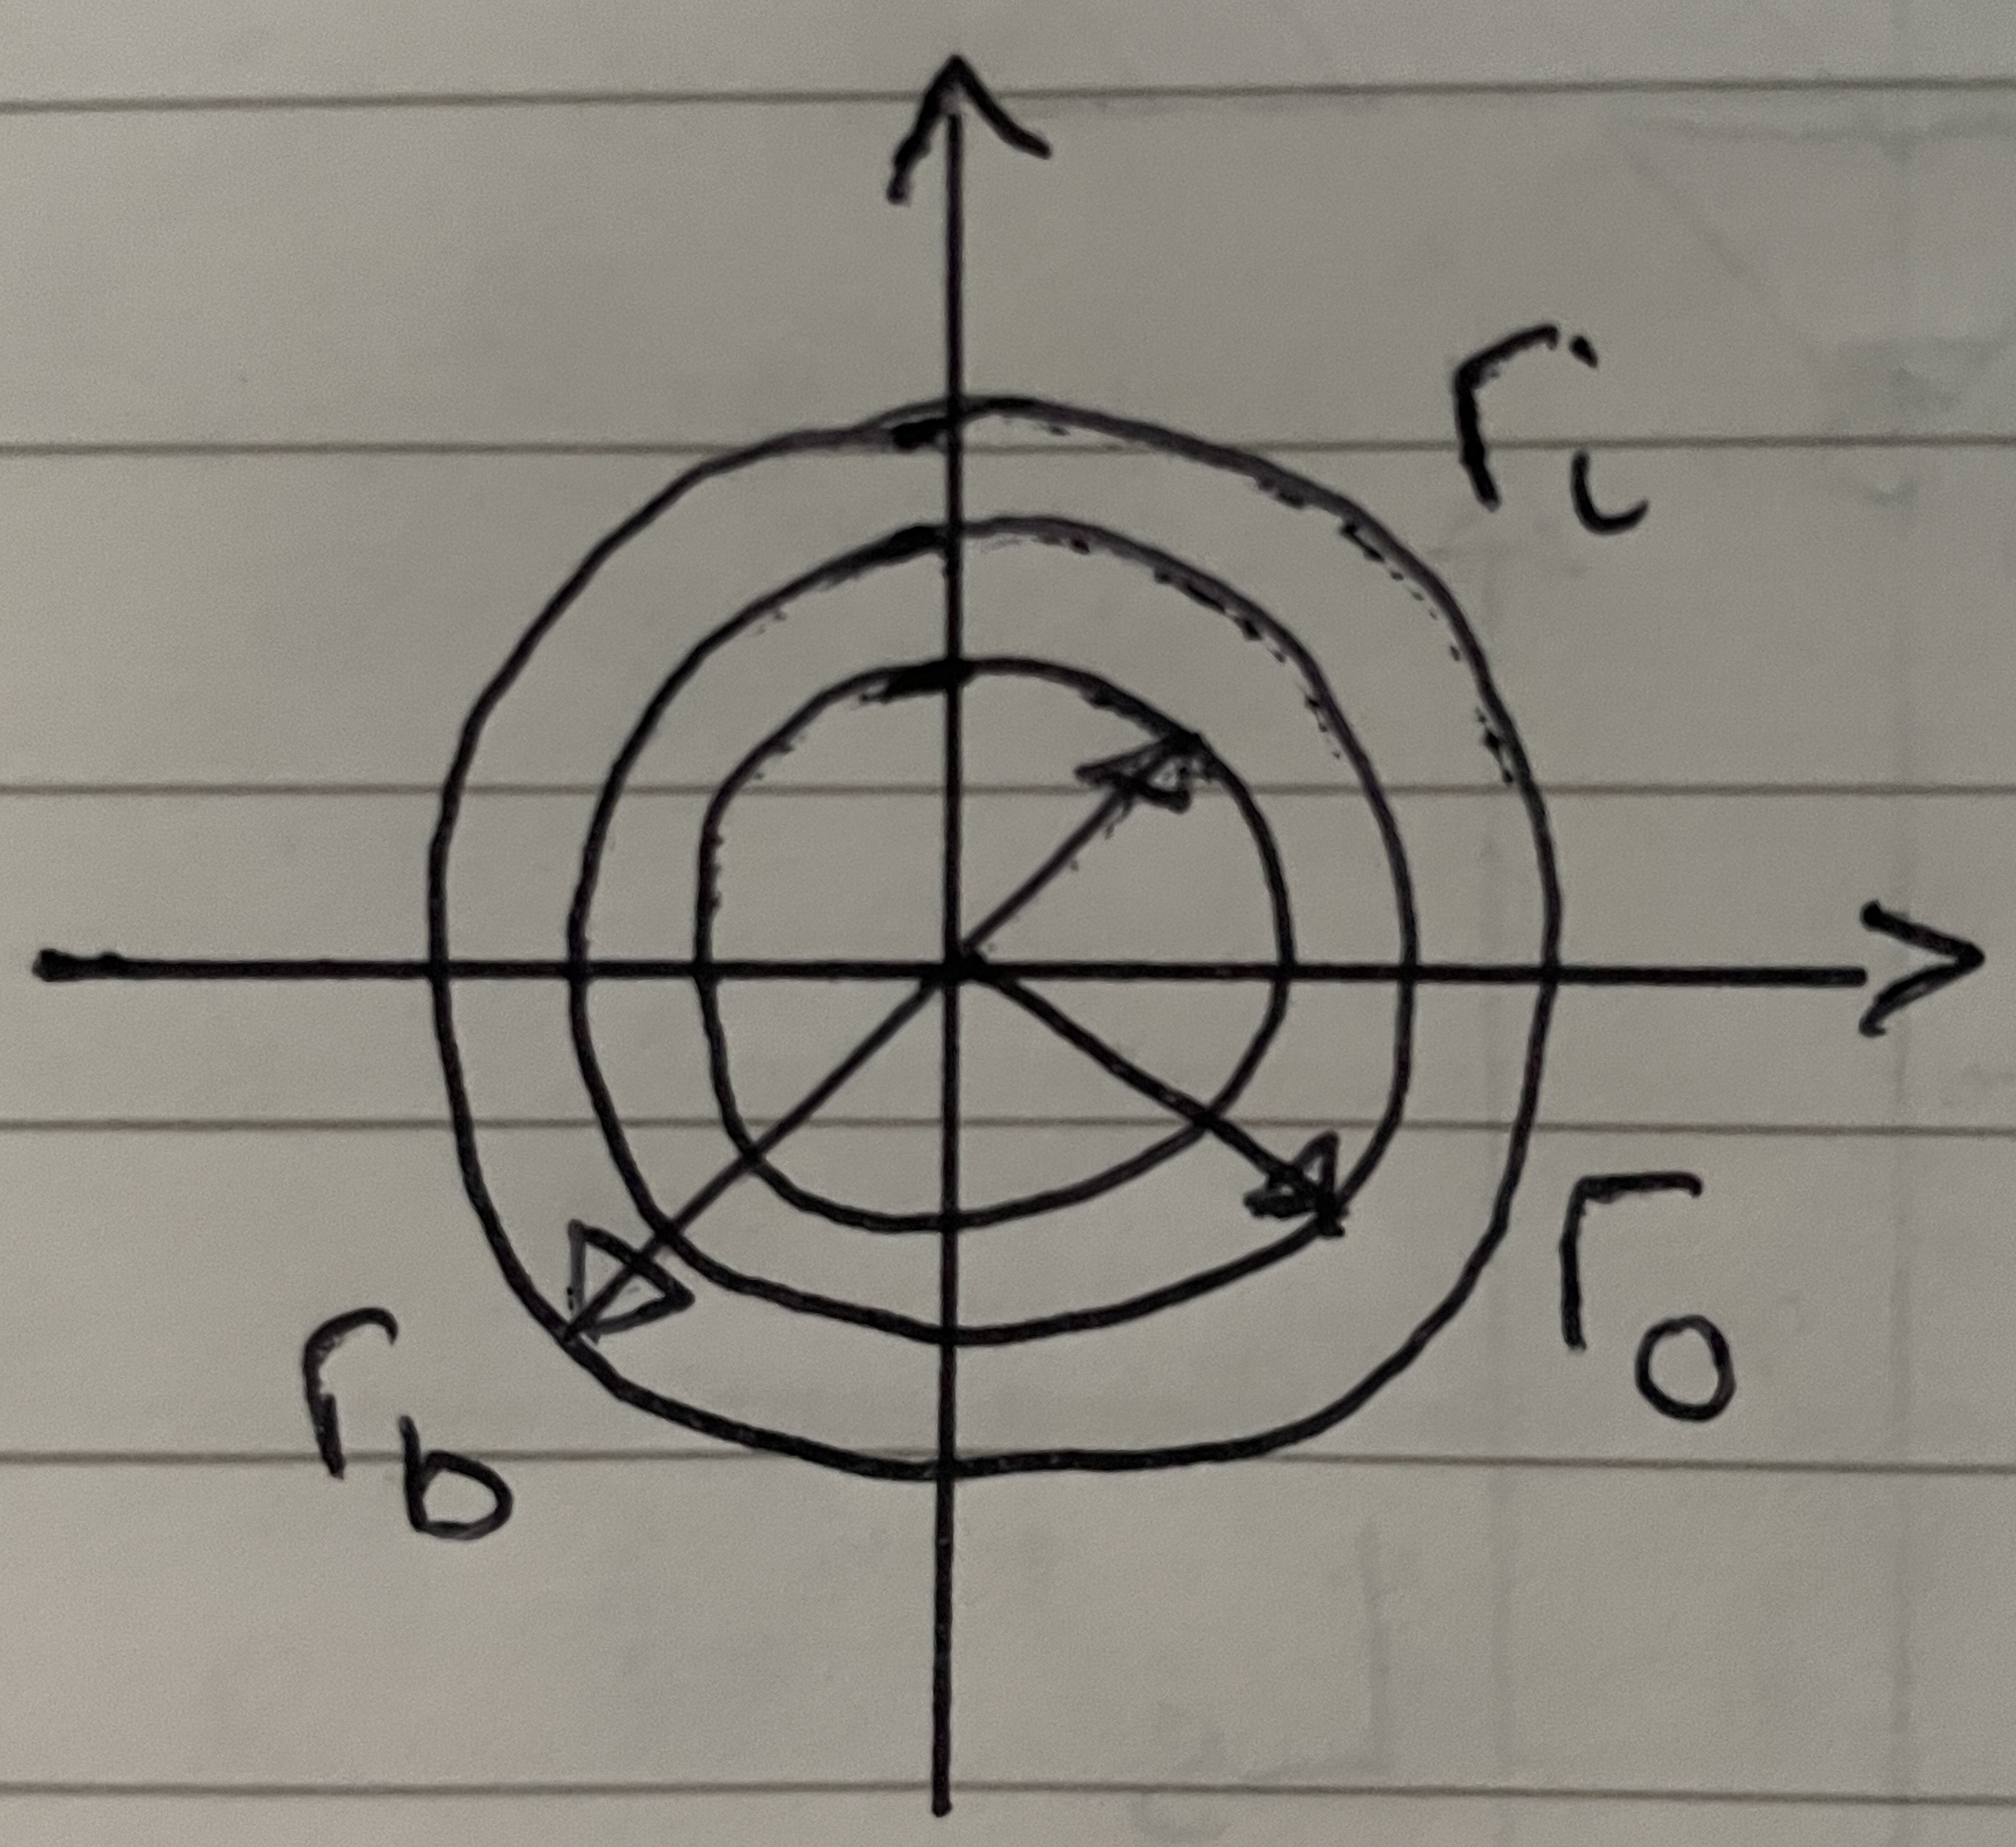
\includegraphics[height =5cm]{./img/q2i2.jpg}
    \caption{Sketch of cylinder arrangement.}
\end{figure}
\begin{figure}[H]
    \centering
    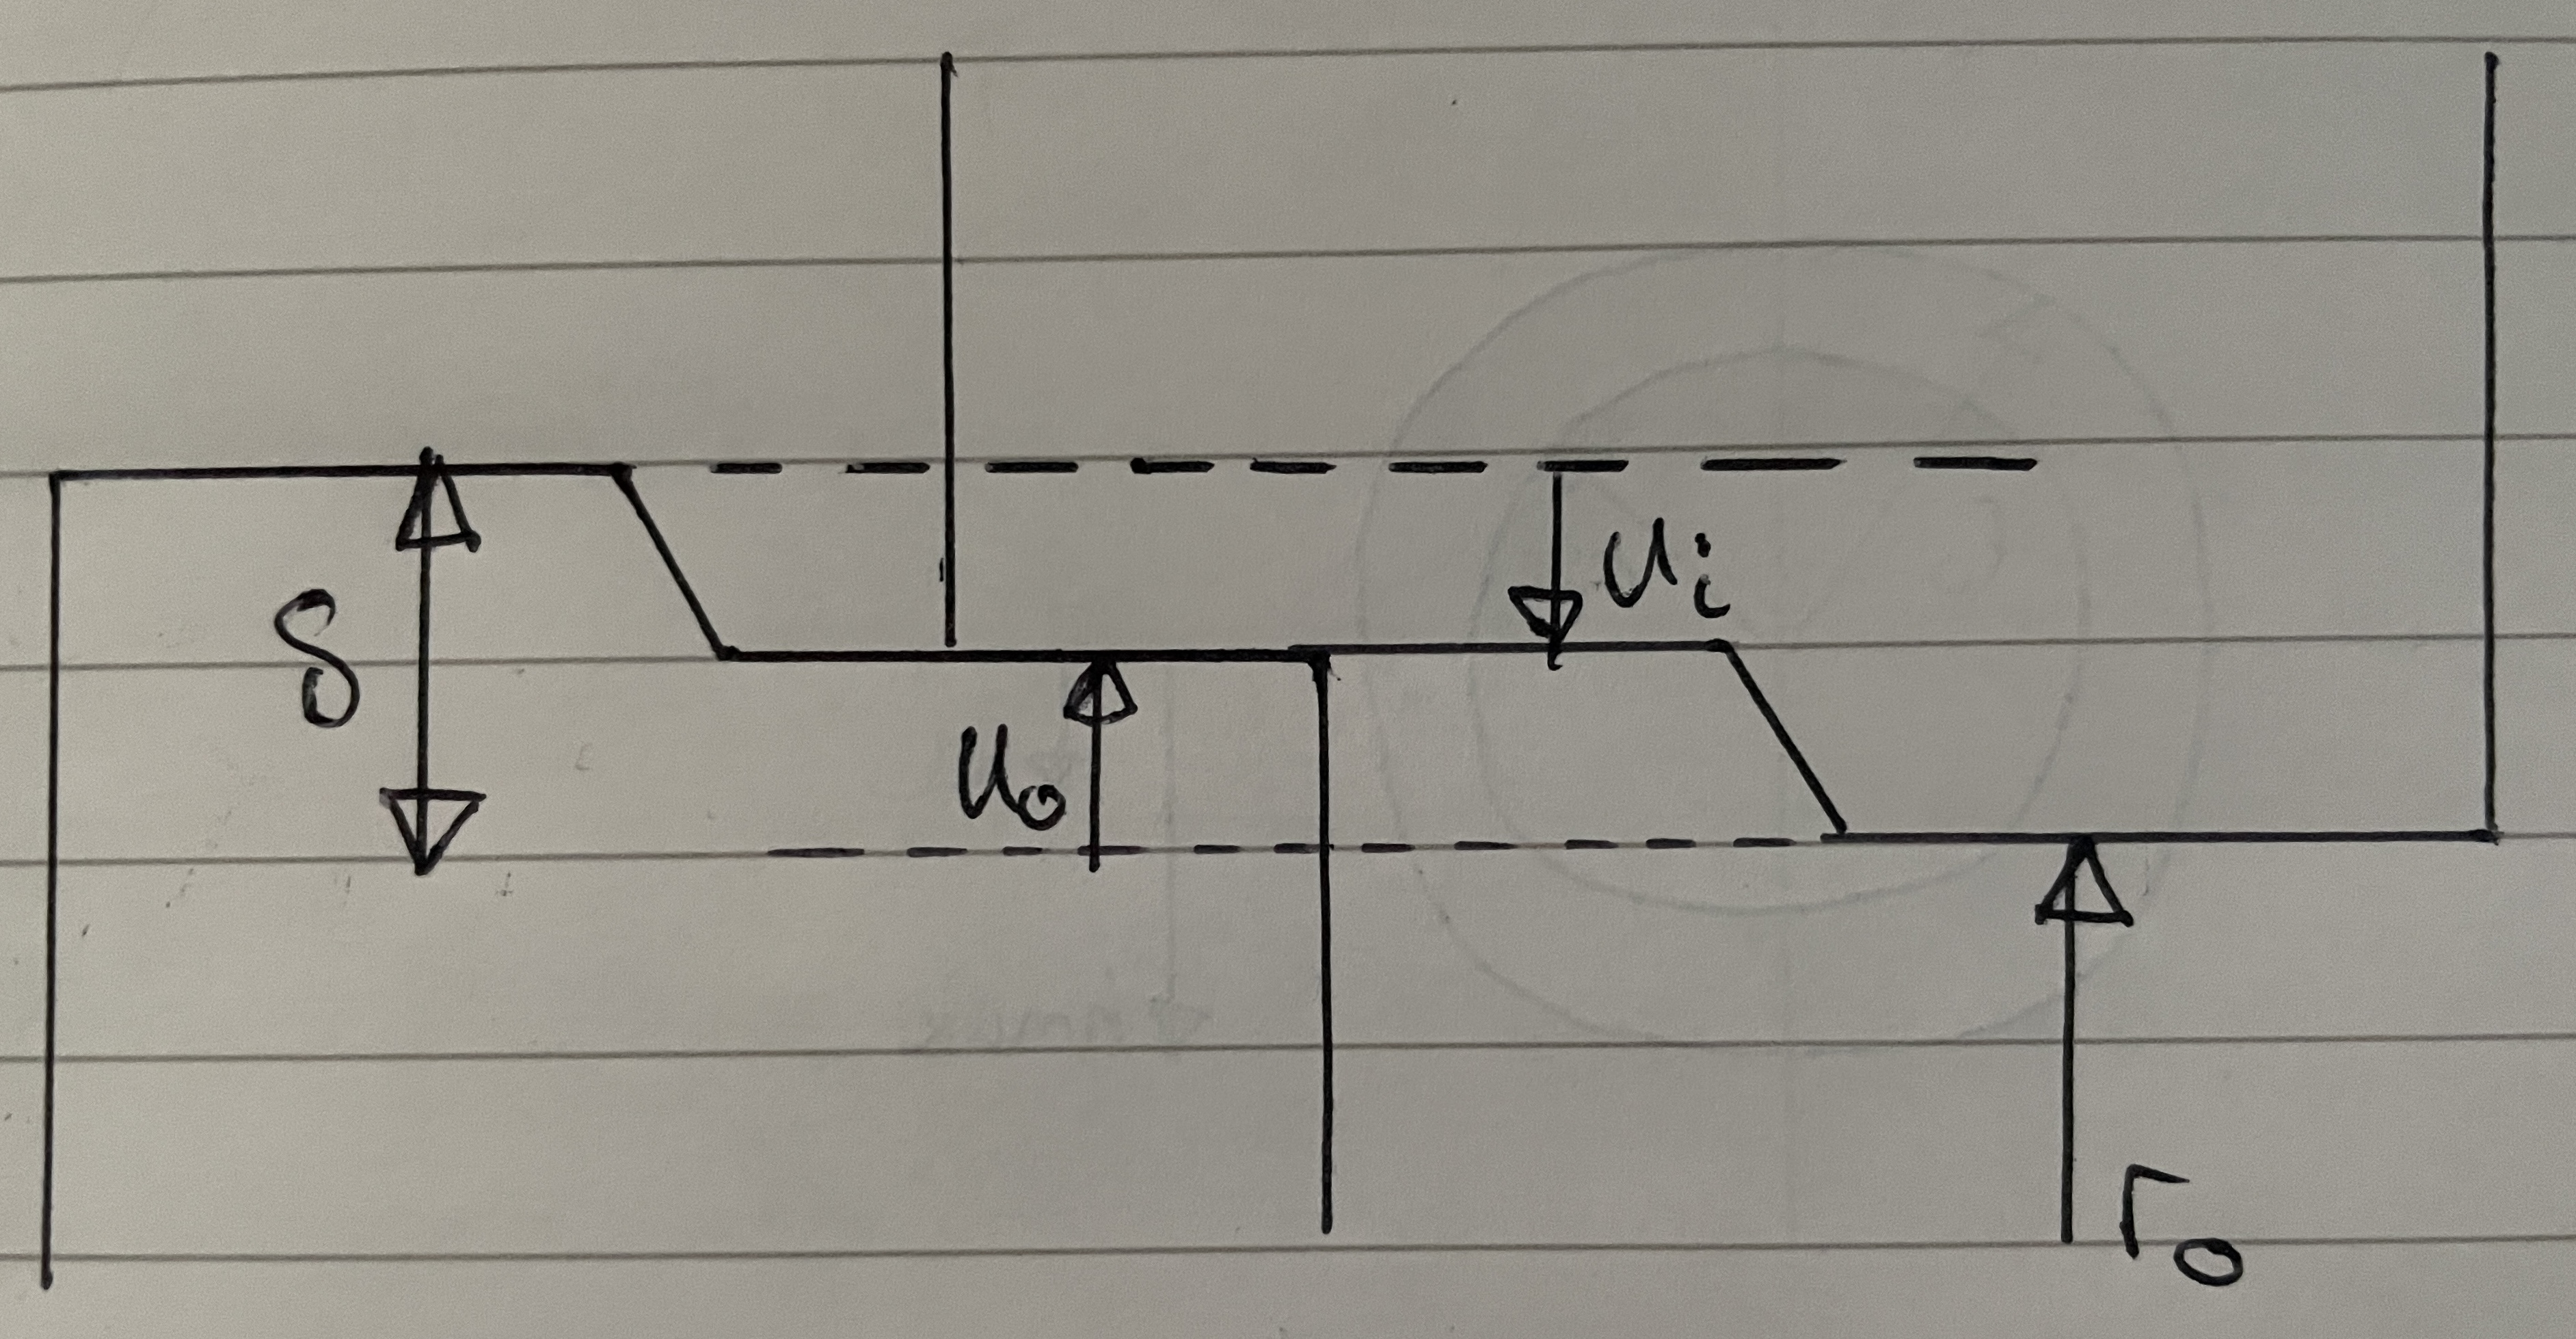
\includegraphics[height =5cm]{./img/q2i1.jpg}
    \caption{Diagram to show interference.}
\end{figure}
Hence:
\begin{equation}
    \delta = u_o - u_i
\end{equation}
Finding $u_i$. Let us start with the general equation for $u$:
\begin{gather}
    u = \frac{r}{E}\left(\sigma_{\theta} - v \sigma_r\right)\\
    \rightarrow u_i = \frac{d_0}{E_i}\left[\sigma_{\theta, i} \left(d_0\right) - v_i \sigma_{r,i} (d_0)\right]
\end{gather}
Lame's equations:
\begin{gather}
    \sigma_r = A - \frac{B}{r^2}\\
    \sigma_{\theta} = A + \frac{B}{r^2}
\end{gather}
Boundary conditions:
\begin{gather}
    \sigma_{r,i}(d_i) = 0 = A - \frac{B}{d_i^2}\\
    \sigma_{r,i}(d_0) - -p_{int} = A - \frac{B}{d_0^2}\\
    A = -p_{int}\frac{d_0^2}{d_0^2 - d_i^2}\\
    B = -p_{int}\frac{d_i^2 \cdot d_0^2}{d_0^2 - d_i^2}
\end{gather}
Substituting:
\begin{equation}
    \sigma_{\theta,i} = A + \frac{B}{r^2} = -p_{int}\frac{d_0^2}{d_0^2 - d_i^2} \left(1 + \frac{d_i^2}{r^2}\right)
\end{equation}
Therefore:
\begin{gather}
    \sigma_{r,i}(d_0) = -p_{int} \hspace{1cm} \sigma_{\theta,i}(d_0) = -p_{int}\frac{d_0^2 + d_i^2}{d_0^2 - d_i^2}\\
    u_i = -p_{int} \frac{d_0}{E_i} \left(\frac{d_0^2 + d_i^2}{d_0^2 - d_i^2} - v_i\right)
\end{gather}
Repeating to find $u_o$:
\begin{gather}
    u_o = \frac{d_0}{E_o}\left[\sigma_{\theta,o} (d_0) - v_o \sigma_{r,o}(d_0)\right]
\end{gather}
Lame's equations:
\begin{gather}
    \sigma_r = A - \frac{B}{r^2}\\
    \sigma_{\theta} = A + \frac{B}{r^2}
\end{gather}
Boundary conditions:
\begin{gather}
    \sigma_{r,o}(d_0) = -p_{int} = A - \frac{B}{d_0^2}\\
    \sigma_{r,o}(d_b) = 0 = A - \frac{B}{d_b^2}\\
    A = -p_{int} \frac{d_0^2}{d_0^2- d_b^2}\\
    B = -p_{int} \frac{d_0^2 \cdot d_b^2}{d_b^2 - d_0^2}
\end{gather}
Substituting:
\begin{gather}
    \sigma_{\theta,o} = A + \frac{B}{r^2} = -p_{int} \frac{d_0^2}{d_b^2 - ^2} \left(1+ \frac{d_b^2}{r^2}\right)
\end{gather}
Therefore:
\begin{gather}
    \sigma_{r,o}(d_b) = 0 \hspace{1cm} \sigma_{\theta,o}(d_0) = p_{int}\frac{d_b^2 + d_0^2}{d_b^2 -d_0^2}\\
    u_o = p_{int} \frac{d_0}{E_o}\left(\frac{d_b^2 + d_0^2}{d_b^2 - d_0^2} + v_o\right)
\end{gather}
Finding $\delta$:
\begin{gather}
    u_i =-p_{int}\frac{d_0}{E_i}\left(\frac{d_0^2 + d_i^2 }{d_0^2 - d_i^2}-v_i\right)\\
    u_o = p_{int}\frac{d_0}{E_o}\left(\frac{d_b^2 + d_0^2 }{d_b^2 - d_0^2}+v_o\right)\\
    \delta = p_{int}d_0\left[\frac{1}{E_o}\left(\frac{d_b^2 + d_0^2}{d_b^2 - d_0^2}+v_o\right) + \frac{1}{E_i}\left(\frac{d_0^2 + d_i^2}{d_0^2 - d_i^2}-v_i\right)\right]
\end{gather}
For a single material: $E_i = E_o = E$, and $v_i = v_o = v$:
\begin{gather}
    \delta = p_{int} \frac{d_0}{E}\left[\frac{2d_0^2\left(d_b^2-d_i^2\right)}{\left(d_b^2 - d_0^2\right)\left(d_0^2-d_i^2\right)}\right]\\
    p_{int} = E \delta \left[\frac{\left(d_b^2 + d_0^2\right)\left(d_0^2 - d_b^2\right)}{2d_0^3\left(d_b^2 - d_i^2\right)}\right]
\end{gather}
\end{document}